\section{Implementacja}
Używana przez nas biblioteka \textit{MultiAgent-Gym} domyślnie dostarcza przykładowe
środowiska, które reprezentują różnego rodzaju problemy (w tym przypadku są to różnego
rodzaju gry, w których agenci konkurują ze sobą).

Do naszych celów konieczne było utworzenie nowego środowiska, korzystając z bazowych elementów biblioteki.
Najistotniejszą zmianą jest sposób uczenia poszczególnych agentów. W przypadku domyślnego
przykładu gry \textit{Predator and Prey} agentami są jedynie łowcy, podczas gdy ofiary poruszają
się losowo. Chcieliśmy jednak zamodelować sytuację dwóch konkurujących zespołów, zatem wprowadziliśmy
następujące modyfikacje:
\begin{itemize}
    \item Każdy aktor jest oddzielnym agentem, z własnym zestawem parametrów
    \item Każdy agent otrzymuje indywidualnie obliczaną nagrodę na podstawie określonych kryteriów
    \item Każdy agent komunikuje się z innymi, przekazując informacje o aktualnie obserwowanym otoczeniu,
          co pozwala całej grupie na podejmowanie decyzji w oparciu o wspólną wiedzę (Rys. \ref{fig:agent_view}).
\end{itemize}
\begin{figure}[H]
  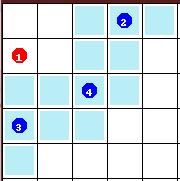
\includegraphics[width=\linewidth]{images/agent_view.png}
  \caption{Obszar widziany przez agenta nr 4.}
  \label{fig:agent_view}
\end{figure}


Niezależnie od siebie agenci podejmują następujące decyzje:
\begin{itemize}
    \item Wykonują optymalny ruch na podstawie obserwacji
    \item Uczą się na podstawie każdej podjętej akcji, obserwacji konsekwencji swoich działań 
          przed i po wykonaniu ruchu oraz otrzymanej nagrodzie
\end{itemize}


\subsection{Learning}
Do nauczania w agnetów w naszej pracy użyliśmy popularnego rozwiązania reinforcement learningu.

\subsection{Funkcja nagrody}
W grze definiujemy funkcję kosztu tury. Koszt wykonania tury w naszym przypadku jest liczbą ujemną. Predatorom
za każdą turę odejmuje się punkty, ponieważ ich celem jest jak najszybsze schwytanie ofiar. Natomiast ofiary otrzymują 
punkty z każdą turą ponieważ w ich celem jest przeżycie jak największej liczby tur.\\

Funkcja nagrody skłąda sie z następujących czynników
\begin{itemize}
    \item Koszt ruchu - oznaczony dalej jako sc (step cost) - globalne zwykle mniejszy 0
    \item Ilość żywych ofiar - oznaczona jako pa (prays alive)
    \item Kara za podejście wyłącznie jednego predatora do ofiary - oznaczona jako p (penalty) - globalne zwykle mniejszy 0 
    \item Nagroda za schwytania ofiary - oznaczone jako cr (capture reward) - globalne zwykle większy 0
    \item Ilość predatorów w najbliższym otoczeniu danej ofiary- oznaczone jako pc (predators count)
\end{itemize}

Nagroda przyznana ofierze w danym ruchu wyraża się w następujący sposób:\\
\begin{algorithm}[H]
 praysAlive = getPraysAlive()\;
 pa = len(praysAlive)\;
 \For{predator in getPredatorsList():}{
    predator.reward = PredatorBaseAward(sc,pa)\;
 }
 \For{pray in praysAlive:}{
    prey.reward  += PreyBaseAward(sc,pa)\;
    pc = countPredatorsAround(prey)\;
    prey.reward  += PreyAdditionalAward(p,cr,pc)\;
    \For{for predator in getPredatorsNeighbourList(prey):}{
        predator.reward +=  PredatorAdditionalAward(p,cr,pc)\;
    }
 }
 \caption{Rewarding algorith}
\end{algorithm}

\\
PreyBaseAward(sc, pa) = sc*pa \\
PredatorBaseAward(sc, pa) = -sc * pa \\
PreyAdditionalAward(p, cr, pc) = \begin{cases}
    \text{if }  pc = 0 & =  0\\
    \text{else if } pc = 1 & = + p \\
    \text{else } pc > 1& = - cr \\
\end{cases}\\
PredatorAdditionalAward(p, cr, pc)= \begin{cases}
    \text{if }  pc = 0 & =  0\\
    \text{else if } pc = 1 & = p \\
    \text{else } pc > 1& = cr/pc \\
\end{cases}








